\chapter{Dielectric Properties of Amorphous Zr-Al-O and Zr-Si-O Thin Films}

{\let\thefootnote\relax\footnote{{
This work was published to \emph{Journal of Advanced Dielectrics}. Reprinted with permission from \cite{Naoi2015}.
}}}

\section{Abstract}
We have systematically studied the composition dependence of the dielectric properties of $\textnormal{Zr}_{1-x}\textnormal{Al}_{x}\textnormal{O}_{2-x/2}$ and $\textnormal{Zr}_{1-x}\textnormal{Si}_{x}\textnormal{O}_{2}$.
An essentially linear variation of the static dielectric constant, $\varepsilon_s$, was observed as a function of composition, $x$, for compositions rich in the p-block element, i.e., $x>0.4$, for both chemical systems. However an abrupt change in $\varepsilon_s$ is found near $x \approx 0.35$, associated with the onset of crystallinity in as-deposited films. Breakdown fields do not show a comparable composition dependence. Measurements of the index of refraction at optical frequencies, combined with a simple Clausius-Mossotti interpretation, indicates that low-frequency (ionic) contributions to the polarizability exhibit systematic deviation with respect to values linearly interpolated from the endmembers. These trends are not consistently affected by the presence of crystalline order, but are related to changes associated with heterogeneous local oxygen coordination and bonding.

\section{Introduction}
Amorphous  dielectrics comprising mixed transition-metal/p-block (e.g., Hf, Zr or Ta combined with Al, Si or Ge) oxides are technologically important and are generally viewed as following simple trends as a function of composition. Some examples (e.g., Zr-Si-O) have been found to exhibit unexpected behavior, such as an enhanced dielectric constant \cite{Wilk2000,Wilk2001,Lucovsky2000,Naoi2012}.
Amorphous \ce{HfO2}-based dielectrics, modified with the addition of \ce{SiO2} and/or \ce{Al2O3}, are now widely used in commercial integrated circuits as alternatives to the native \ce{SiO2} dielectric that controls charge transport in Si-channel field-effect transistors, because \ce{HfO2}, like other oxides of the Group 3, 4, and 5 elements, has a significantly higher dielectric constant (static value of the relative dielectric constant, $\varepsilon_s = \varepsilon (\omega \rightarrow 0)/\varepsilon_0 \approx 23$) than \ce{SiO2} for which $\varepsilon_s \approx 3.9$. 
Compared to \ce{SiO2} they can therefore achieve a comparable charge density at a specified gate voltage using a layer thick enough to avoid excessive leakage by direct tunneling \cite{Kingon2000}. Ab-initio studies of amorphous $\textnormal{Zr}_{1-x}\textnormal{Si}_{x}\textnormal{O}_{2}$ and $\textnormal{Hf}_{1-x}\textnormal{Si}_{x}\textnormal{O}_{2}$ and related materials have highlighted the importance of local structure on dielectric properties, and the consequent impact on the composition dependence \cite{Pignedoli2007,Nakamura2005,Rignanese2002,Ouyang2005}.

In order to understand the behavior of this interesting class of materials, we have focused on the Zr-Al-O and Zr-Si-O systems. Films deposited at room temperature exhibit a clear transition from nanocrystalline (Zr-rich compositions) to amorphous (Si- or Al-rich compositions). Polycrystalline and amorphous thin films of these materials exhibit comparable values for $\varepsilon_{s}$; in both case the value represents an approximate directional average of the anisotropic value associated with single crystals. The question of crystallinity can be important; for example, as gate dielectrics, amorphous oxides are advantageous over polycrystalline materials since they avoid inhomogeneity in local charge density due to anisotropy that would degrade mobility in the conducting channel of an FET. Polycrystalline dielectrics are expected to exhibit a lower breakdown field than that of amorphous dielectrics due to the presence of grain boundaries \cite{Lanza2012}. %=reference suggesting grain boundaries lead to low breakdown
We are using these two systems to determine the effect of the presence or absence of crystallinity on the dielectric constant and the breakdown field, and to determine the systematic effect of the Zr/Si or Zr/Al ratio on these properties. This information provides insight regarding the mechanism for the observed enhancement of the dielectric response. 

We used a composition-spread technique for thin film growth to enable composition-dependent trends to be identified with low composition-to-composition process variation and very fine composition resolution. The dielectric constant of amorphous films was found to vary roughly linearly with composition, while the static dielectric constant of crystalline (transition-metal-rich) films was found to be significantly higher. Leakage currents and breakdown fields were less strongly composition dependent and suggest that grain boundaries in nanocrystalline samples do not serve as weak links.

\section{Experimental Methods}
%Sputtering
Compositionally-graded films were prepared using 90$\degree$
off-axis reactive cosputtering using two 2-inch planar magnetron sputter guns arranged in a facing-targets configuration,
as described previously \cite{vanDover1999}.
The 75 mm diameter Si substrates were positioned
between the two guns so that species sputtered from each
target condense on the substrate simultaneously. The
deposition rate decreases rapidly as a function of distance from
the target, so a natural composition gradient is obtained in this geometry \cite{vanDover1999}.
The sputter guns were operated at rf power levels chosen to achieve approximately 1:1 cation ratio at the center of the substrate.
The films were about 100 nm thick with cations randomly mixed on an atomic scale. Films used for evaluation of crystallinity were deposited on bare Si wafers while those used for evaluation of electrical and optical properties were deposited on wafers pre-coated with sputtered TiN).
Prior to film deposition the vacuum chamber was evacuated to a pressure of 10$^{-6}$ Torr or lower.  Gas flow rates during deposition were 15 std. $\textnormal{cm}^3 / \textnormal{minute}$ (sccm) Ar and 10 sccm \ce{O2}, with the turbopump throttled to maintain a pressure of 30 mTorr in the chamber.  
The substrate was also intentionally biased with 10 W rf power, yielding a dc potential of -75 V that ensures formation of a dense film (avoiding formation of columnar voids during deposition \cite{Barron2009}.)
The substrate temperature during deposition was maintained below 60 \textdegree C by attaching the substrate to a heatsink. Under these conditions the deposition rate was roughly 0.1 nm/s,though the rate varies somewhat with position on the sample.  The final thickness of the films was on the order of 100 nm.  

%composition
The composition of the films intentionally varies along the length of the sample.  Quantitative composition variation was determined using calibration samples on which a single element was reactively sputtered under the same conditions used for the cosputtered spreads.  The thickness of the deposited film, measured as a function of position using a profilometer, was used to calculate the deposition rate.  The cation composition of the cosputtered sample is then inferred simply by calculating the ratio of arrival rates of the two cation species.  The oxygen stoichiometry in these systems was calculated using charge balance assuming cations are in their highest oxidation state, an assumption that is validated by the observation of low leakage currents in the dielectric. An example of the position dependence of composition is shown in Fig. \ref{ZrAlO_compositions_RBS}.  At selected positions the codeposited samples were examined using Rutherford Backscattering Spectroscopy (RBS).  The RBS analysis, which has an absolute accuracy estimated to be better than 5\%, yielded compositions that were consistent with the results of the rate calibrations, confirming the validity of all of the assumptions inherent in the latter technique.  A typical RBS spectrum is shown in the inset to Fig. \ref{ZrAlO_compositions_RBS}.

The thickness of the films is not strictly constant across the length of the sample, since the sum of the deposition rates from the two targets is not constant.  The thickness was therefore determined as a function of position by preparing a codeposited sample with a liftoff mask.  The mask was then removed and the thickness of the deposited film was determined at fifteen positions using a profilometer.  These measurements of the dependence of thickness with position were interpolated using a quadratic fit.

\begin{figure}
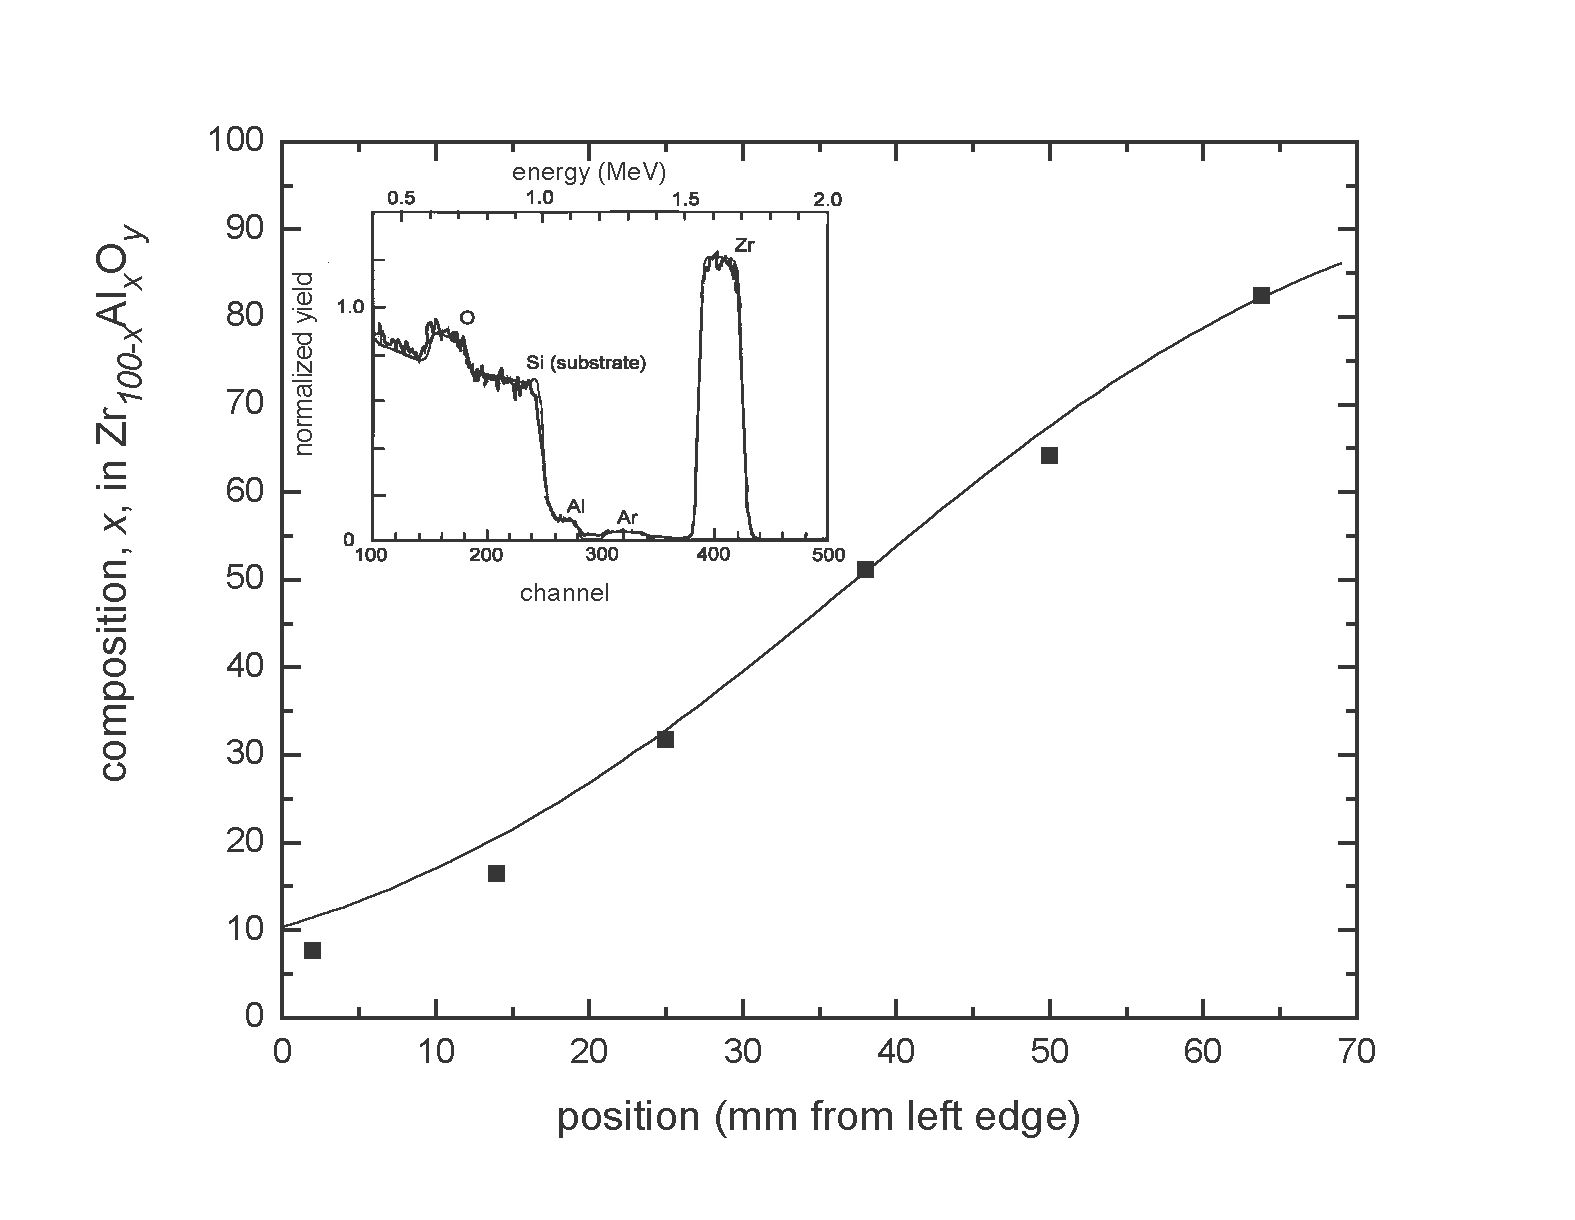
\includegraphics[width=\linewidth]{chapter_3/ZrAlO_compositions_RBS}
\caption{Composition as a function of position along the 7-cm sample axis.  Solid line: compositions calculated using rate calibrations for each species (\ce{ZrO2}, \ce{Al2O3}).  Squares: Compositions inferred using Rutherford Backscattering Spectroscopy.  Inset: a typical RBS spectrum used to determine the composition. A small level of Ar incorporation is typical in sputtered films, and can be seen in the RBS spectrum, though it has a negligible effect on electrical or structural properties.}
\label{ZrAlO_compositions_RBS}
\end{figure}
%XRD
X-ray diffraction patterns were taken with a Brucker-AXS system equipped with a Cu $K_\alpha$ generator and crossed-wire area (two-dimensional) detector.
The resulting data were integrated over the range -47$\degree$ $ < \chi < $ -133$\degree$ to yield a single graph of integrated intensity versus $2\theta$. 
The crystallites exhibited no preferred orientation. 
Fig. \ref{ZrAlO_ZrSiO_XRD} illustrates the reflections associated with monoclinic \ce{ZrO2}, observed for Zr-rich compositions that exhibit nanoscale crystalline order.
The width of the peaks, corrected for instrument resolution, is a measure of the crystallite size (structural coherence length, $L$) as inferred using the Debye-Scherrer formula, $L = 0.6 \lambda / B cos \theta$, where $B$ is the full width at half maximum.  
The pattern corresponding to $\textnormal{Zr}_{0.75}\textnormal{Si}_{0.25}\textnormal{O}_{2}$ is marked with the $(hkl)$ Miller indices of the monoclinic phase; the distinct peak expected for cubic or tetragonal \ce{ZrO2} at approximately 30$\degree$ is clearly not present in the pattern. 
The pattern corresponding to $\textnormal{Zr}_{0.89}\textnormal{Al}_{0.11}\textnormal{O}_{1.94}$ is less well defined, but is consistent with monoclinic \ce{ZrO2}.
It is surprising that the monoclinic phase should be present in nanocrystalline $\textnormal{Zr}_{0.89}\textnormal{Al}_{0.11}\textnormal{O}_{1.94}$, both because incorporation of a trivalent ion in \ce{ZrO2} introduces O vacancies that typically stabilize the cubic fluorite phase, as in yttrium-stabilized zirconia, and because grain refinement in unsubstituted \ce{ZrO2} also stabilizes the cubic phase \cite{Gupta}.
When an identical $\textnormal{Zr}_{1-x}\textnormal{Al}_{x}\textnormal{O}_{2-x/2}$ composition spread was annealed at 1000 \textdegree C for 20 seconds in \ce{N2}, Zr-rich compositions ($x<0.18$) exhibited a mixture of monoclinic and tetragonal phases while for $0.18 < x < 0.40$ the structure was entirely cubic, a result that is not inconsistent with expected equilibrium behavior. For $x>0.4$ a mixture of cubic and amorphous material was present.
Annealing  $\textnormal{Zr}_{1-x}\textnormal{Si}_{x}\textnormal{O}_{2}$ at 1000\textdegree C yielded surprisingly similar results, considering that tetravalent Si will not introduce O vacancies to maintain charge balance. 
Zr-rich compositions ($x<0.35$) exhibited a mixture of monoclinic and tetragonal phases while for $0.35 < x < 0.80$ the structure is entirely cubic. 
Apparently introduction of Si, which favors tetrahedral coordination with O (rather than the octahedral coordination of \ce{ZrO2}), disrupts the interactions that stabilize the monoclinic structure. Interestingly, no evidence for formation of zircon, \ce{ZrSiO4}, is observed in the annealed films \cite{VanDover2003}.     
%
\begin{figure}
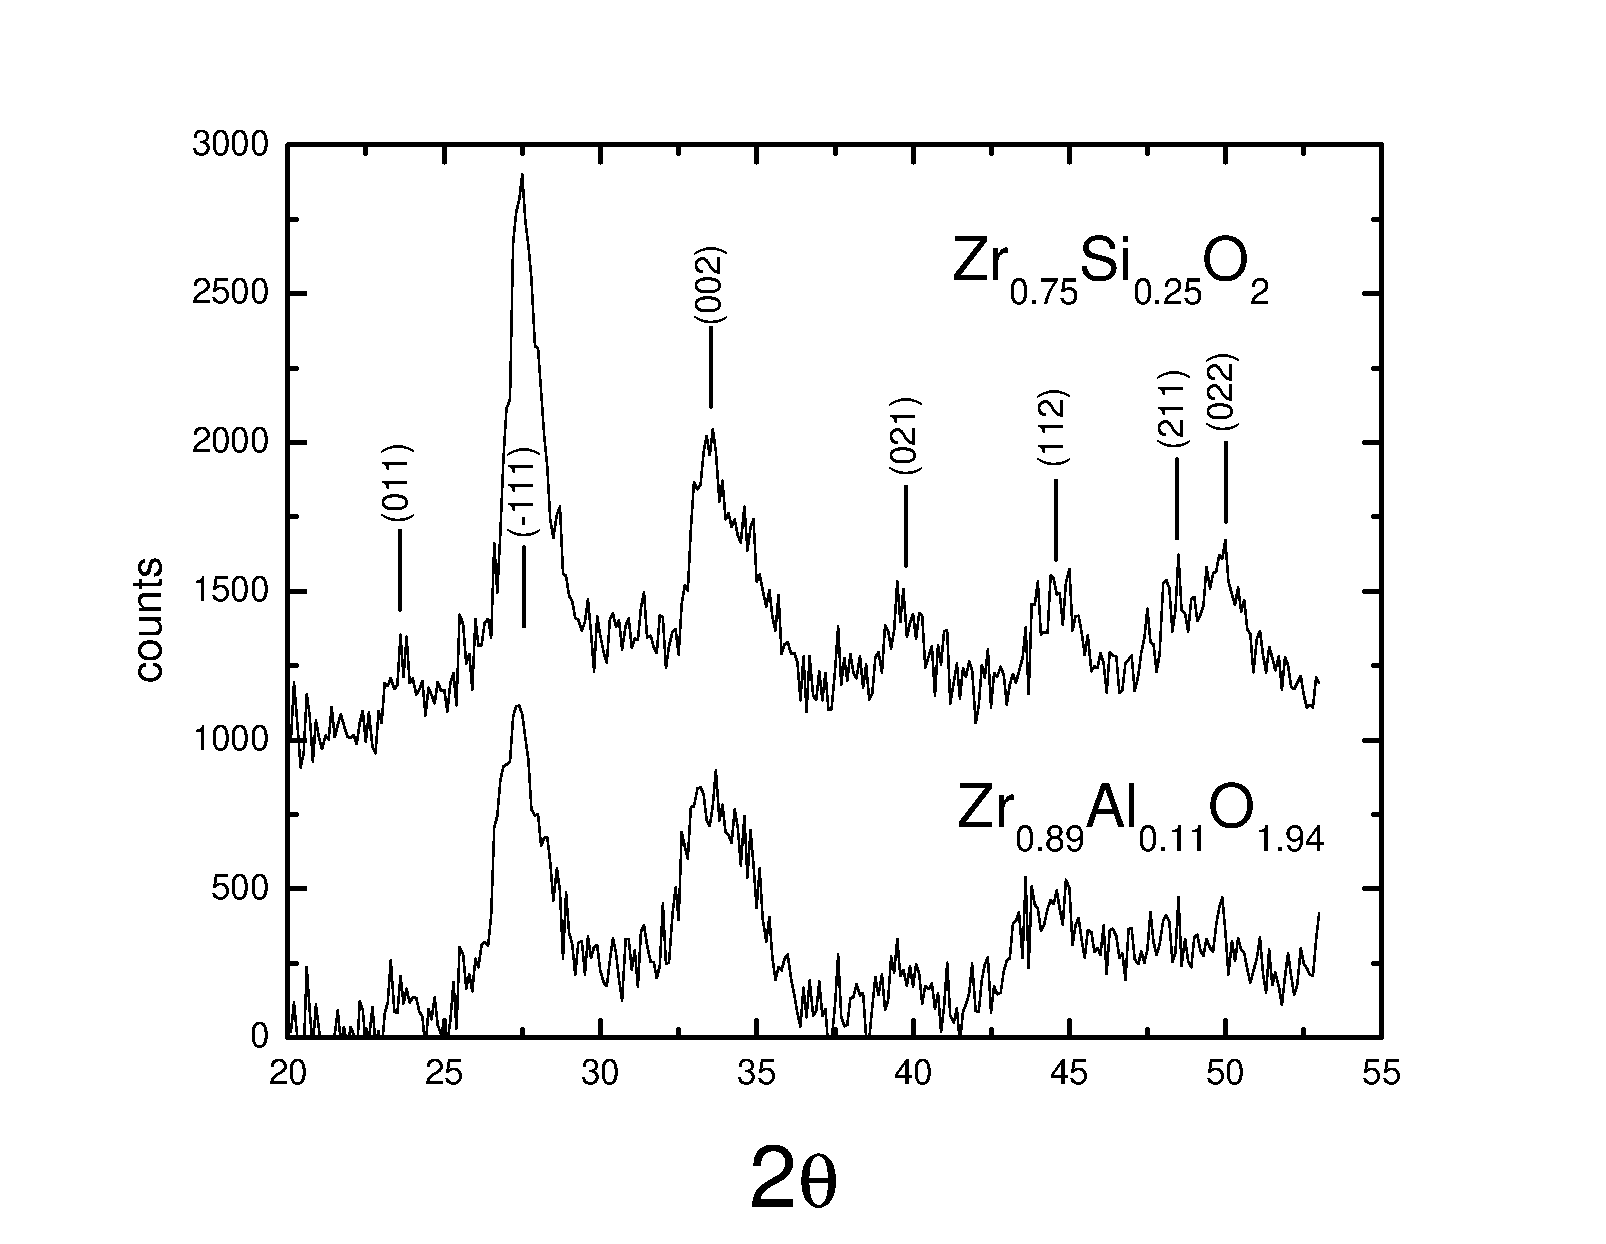
\includegraphics[width=\linewidth]{chapter_3/ZrAlO_ZrSiO_XRD}
\caption{X-ray diffraction patterns for typical nanocrystalline Zr-rich samples. Top curve:  $Zr_{0.75}Si_{0.25}O_2$ film as deposited, offset vertically for clarity, with positions for the strongest monoclinic reflections indicated. Bottom curve: $Zr_{0.89}Al_{0.11}O_{1.94}$, illustrating x-ray peaks that are broader due to the lower degree of crystallinity compared to the Zr-Si-O sample.}
\label{ZrAlO_ZrSiO_XRD}
\end{figure}	


%Ellipsometry
The index of refraction and thickness of the films were determined using a Sentech SE801 spectroscopic ellipsometer over a wavelength range of 450-800 nm. The optical constants of the substrate layer were determined prior to film deposition and were fixed during the fitting process. A film/substrate bilayer model was used to fit $\psi$ and $\delta$, and the optical constants of the film were modeled using the Cauchy relation $n(\lambda) =  n_0 + n_1 / \lambda^{2} + n_2 / \lambda^{4}$ using a least-squares routine. The reported refractive index $n$ was taken to be $n_{0}$, i.e., the infinite wavelength limit far from absorption edge.
%

%Electical properties
The static dielectric constant, $\varepsilon_s$ was evaluated using parallel-plate capacitors fabricated on oxide films grown on a non-reactive TiN base electrode.  Pt counterelectrodes 20 nm thick and 200 $\mu$m in diameter were deposited on the films using electron-beam evaporation through a shadow mask.  
The capacitance of these structures was measured at 10 kHz using an automated probing station and an HP4192A capacitance meter.  Some capacitors were measured from 100 Hz to 1 MHz, and were found to exhibit little dispersion over this range. The dissipation factor for all compositions was found to be low ($\tan\delta < 0.05$), indicating high quality films with no anomalous polarization modes \cite{Barron2009}.
Typically 10 to 40  capacitors were measured at each composition in the linear composition spread; the median value was chosen as representative.
Current-voltage characteristics were also measured on the Pt/dielectric/TiN capacitor structures. 
A Keithley 617 source/electrometer was used to apply a stepped voltage across the capacitor and to measure the resulting leakage current. 
Fields from 0 to 10  MV/cm were applied (Pt counterelectrode biased positively), and current densities in the range $10^{-7}$ -- $10^{-3} A/cm^{2}$ were measured.  The breakdown field, $E_{br}$, was defined as the field at which the current density increased by a factor of 100 or more in a single ~0.1 MV/cm step. 
In cases where the I-V curve was continuous even up to $10^{-3} A/cm^2$ (soft breakdown), the breakdown criterion was chosen to simply be the field at which the current density passed $10^{-4} A/cm^2$. 
Again, 10 to 40 capacitors were measured at each composition; because random defects are unavoidable in films fabricated and processed in a non-cleanroom facility we chose the maximum measured $E_{br}$ as the best representative of the intrinsic behavior of the dielectric.

\section{Results and Discussion}
\subsection{Dielectric constant and refractive index}
The composition dependence of the dielectric constant of $\textnormal{Zr}_{\textnormal{x}}\textnormal{Al}_{\textnormal{1-x}}\textnormal{O}_{\textnormal{1.5+x/2}}$ is presented in Fig.
\ref{ZrAlO_epsilon_cohere}. 
Marks at $x=0$ and $x=1.0$ represent expected values for the endmembers. The dielectric constant of \ce{Al2O3} ($\varepsilon_s \approx 9$) is not controversial \cite{Shannon1993a}.
The dielectric constant of monoclinic \ce{ZrO2} appears to be $\varepsilon_s \approx 32$ based on extrapolation of data measured on polycrystalline ceramic (Zr,Y)O$_{\textnormal{x}}$ as reported by Henn, et al. \cite{Henn1995}.
We note that another reference suggests $\varepsilon_s \approx 17$ based on interpretation of infrared spectroscopy \cite{Feinberg}
and supported by first-principles calculations \cite{Zhao2002}.
We note also that these calculations predict that metastable phases of \ce{ZrO2} would have distinctly different values for $\varepsilon_s$, namely $\varepsilon_s \approx 37$ and $\varepsilon_s \approx 47$ for the cubic and monoclinic phases \cite{Zhao2002}.
Other \emph{ab initio} calculations \cite{Vanderbilt2005} predict a value $\varepsilon \approx 21$ for amorphous \ce{ZrO2}
which we have marked on the left-hand axis. 
 
The dielectric constant for amorphous (Al-rich) compositions follows a nearly linear interpolation between the values for the amorphous endmembers. A clear jump in $\varepsilon_s$ is seen at approximately $x=0.35$. 
The transition is associated with the change in crystallinity, as suggested by the top panel of Fig. \ref{ZrAlO_epsilon_cohere}, which reports the XRD coherence length (grain size) as a function of composition: the as-deposited films are completely amorphous for $x \gtrsim 0.35$.
Extrapolating data for $x<0.30$ to the left-hand axis yields a value in good agreement with that inferred for monoclinic \ce{ZrO2}.

\begin{figure}
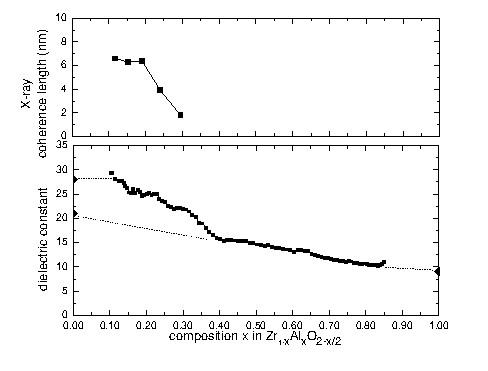
\includegraphics[width=\linewidth]{chapter_3/ZrAlO_epsilon_coherence_1}
\caption{Bottom: Composition dependence of the dielectric constant of thin film $\textnormal{Zr}_{1-x}\textnormal{Al}_{x}\textnormal{O}_{1.5+x/2}$ deposited at room temperature. 
Dotted lines represent extrapolations to values for the endmembers (crystalline and amorphous \ce{ZrO2} and amorphous \ce{Al2O3}) indicated with triangles.Top: composition dependence of the structural coherence length (i.e., essentially grain size) as inferred from X-ray diffraction data using the Debye-Scherrer formula. }
\label{ZrAlO_epsilon_cohere}
\end{figure}

The $\textnormal{Zr}_{1-x}\textnormal{Si}_{x}\textnormal{O}_{2}$ system exhibits a similar behavior as illustrated in Fig. \ref{ZrSiO_eps_cohere}. 
Although the dielectric constant exhibits a nearly linear trend with composition for amorphous compositions ($0.35 < x < 0.90$) and the trend extrapolates to the measured value for \ce{SiO2} ($\varepsilon_s = 3.9$), for $x = 0$ it extrapolates to $\varepsilon_s = 24$ rather than the measured value for amorphous \ce{ZrO2}. 
As in the Zr-Al-O system the abrupt transition in the trend of $\varepsilon_s$ with composition at $x \approx 0.35$ is associated with the change from crystalline to amorphous structure (Fig. \ref{ZrSiO_eps_cohere}, top panel).  
At $x = 0$ the extrapolation of the trend exhibited by crystalline compositions of both Zr-Si-O and Zr-Al-O yields the same value, $\varepsilon_s = 30$, for both, suggesting a common origin. 
However, we note that the crystal structure observed in these films is not the cubic structure bulk \ce{ZrO2} described by Scott, which also extrapolates to $\varepsilon_s = 30$ for undoped \ce{ZrO2}, perhaps coincidentally.   

\begin{figure}
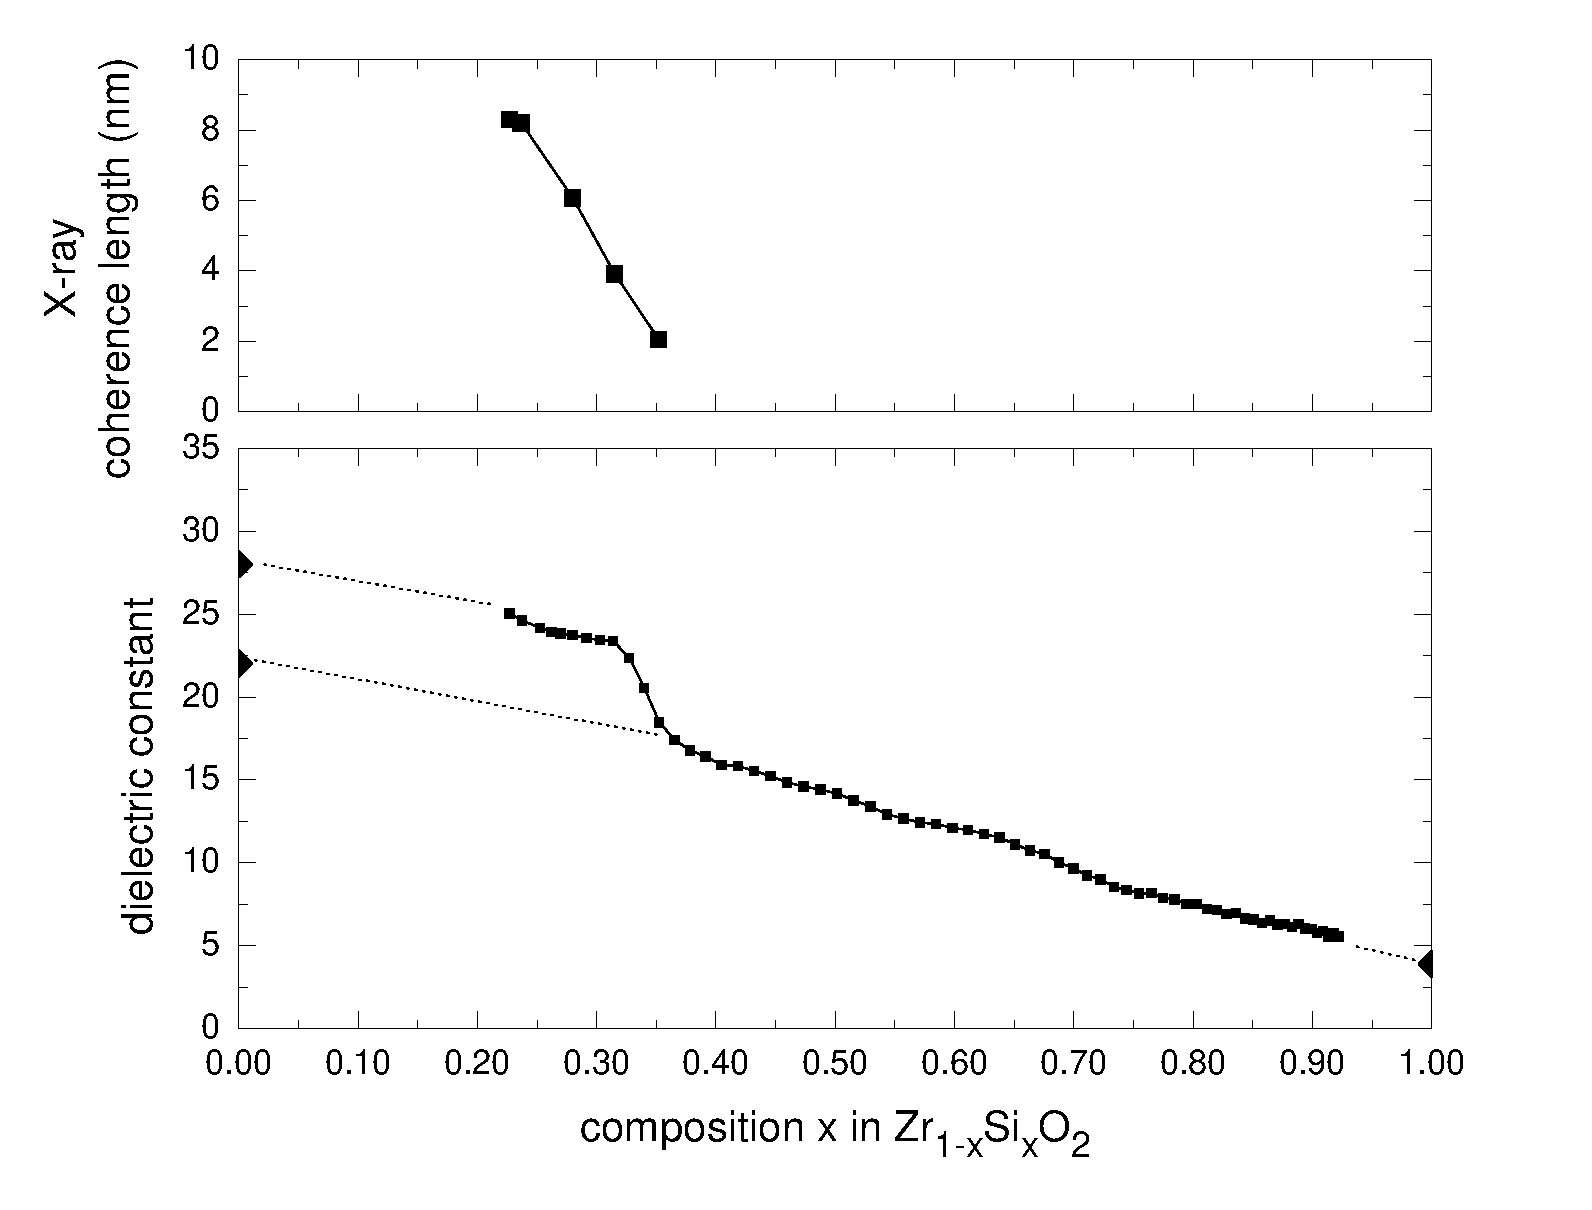
\includegraphics[width=\linewidth]{chapter_3/ZrSiO_epsilon_coherence.pdf}
\caption{Bottom: Composition dependence of the dielectric constant of thin film $\textnormal{Zr}_{1-x}\textnormal{Si}_{x}\textnormal{O}_{2}$ deposited at room temperature. Dotted lines represent extrapolations to values for the endmembers (crystalline and amorphous \ce{ZrO2} and amorphous \ce{SiO2}) indicated with triangles.Top: composition dependence of the structural coherence length (i.e., essentially grain size) as inferred from X-ray diffraction data using the Debye-Scherrer formula.}
\label{ZrSiO_eps_cohere}
\end{figure}

The major trend in dielectric constant as a function of composition in these systems is undoubtedly due to a change in the polarizability from the small values associated with \ce{SiO2} or \ce{Al2O3} to the large value associated with \ce{ZrO2}.  
But it is not immediately evident what fraction of the low-frequency polarizability can be attributed to ionic motion as opposed to polarization of the electrons with respect to atom cores, nor to what degree the density of the film plays a role. 
Fig. \ref{ZrAlO_ZrSiO_index} presents the composition dependence of the index of refraction in these systems. 
The data for $\textnormal{Zr}_{1-x}\textnormal{Al}_{x}\textnormal{O}_{2-x/2}$ follow a smooth trend that extrapolates almost linearly to accepted values for the endmembers \cite{Zhao2002,Kijima2000}.
The data for $\textnormal{Zr}_{1-x}\textnormal{Si}_{x}\textnormal{O}_{2}$ exhibits a more dramatic variation, extrapolating linearly to the endmember value for amorphous \ce{SiO2}. The data are insufficient to allow unambiguous extrapolation to \ce{ZrO2}, though they are consistent with the same value as inferred for $\textnormal{Zr}_{1-x}\textnormal{Al}_{x}\textnormal{O}_{2-x/2}$. 
Where the data for Zr-Al-O show only a break in slope associated with the crystalline-amorphous transition, the data for Zr-Si-O exhibit a jump similar to that observed in the static dielectric constant.    
%
\begin{figure}
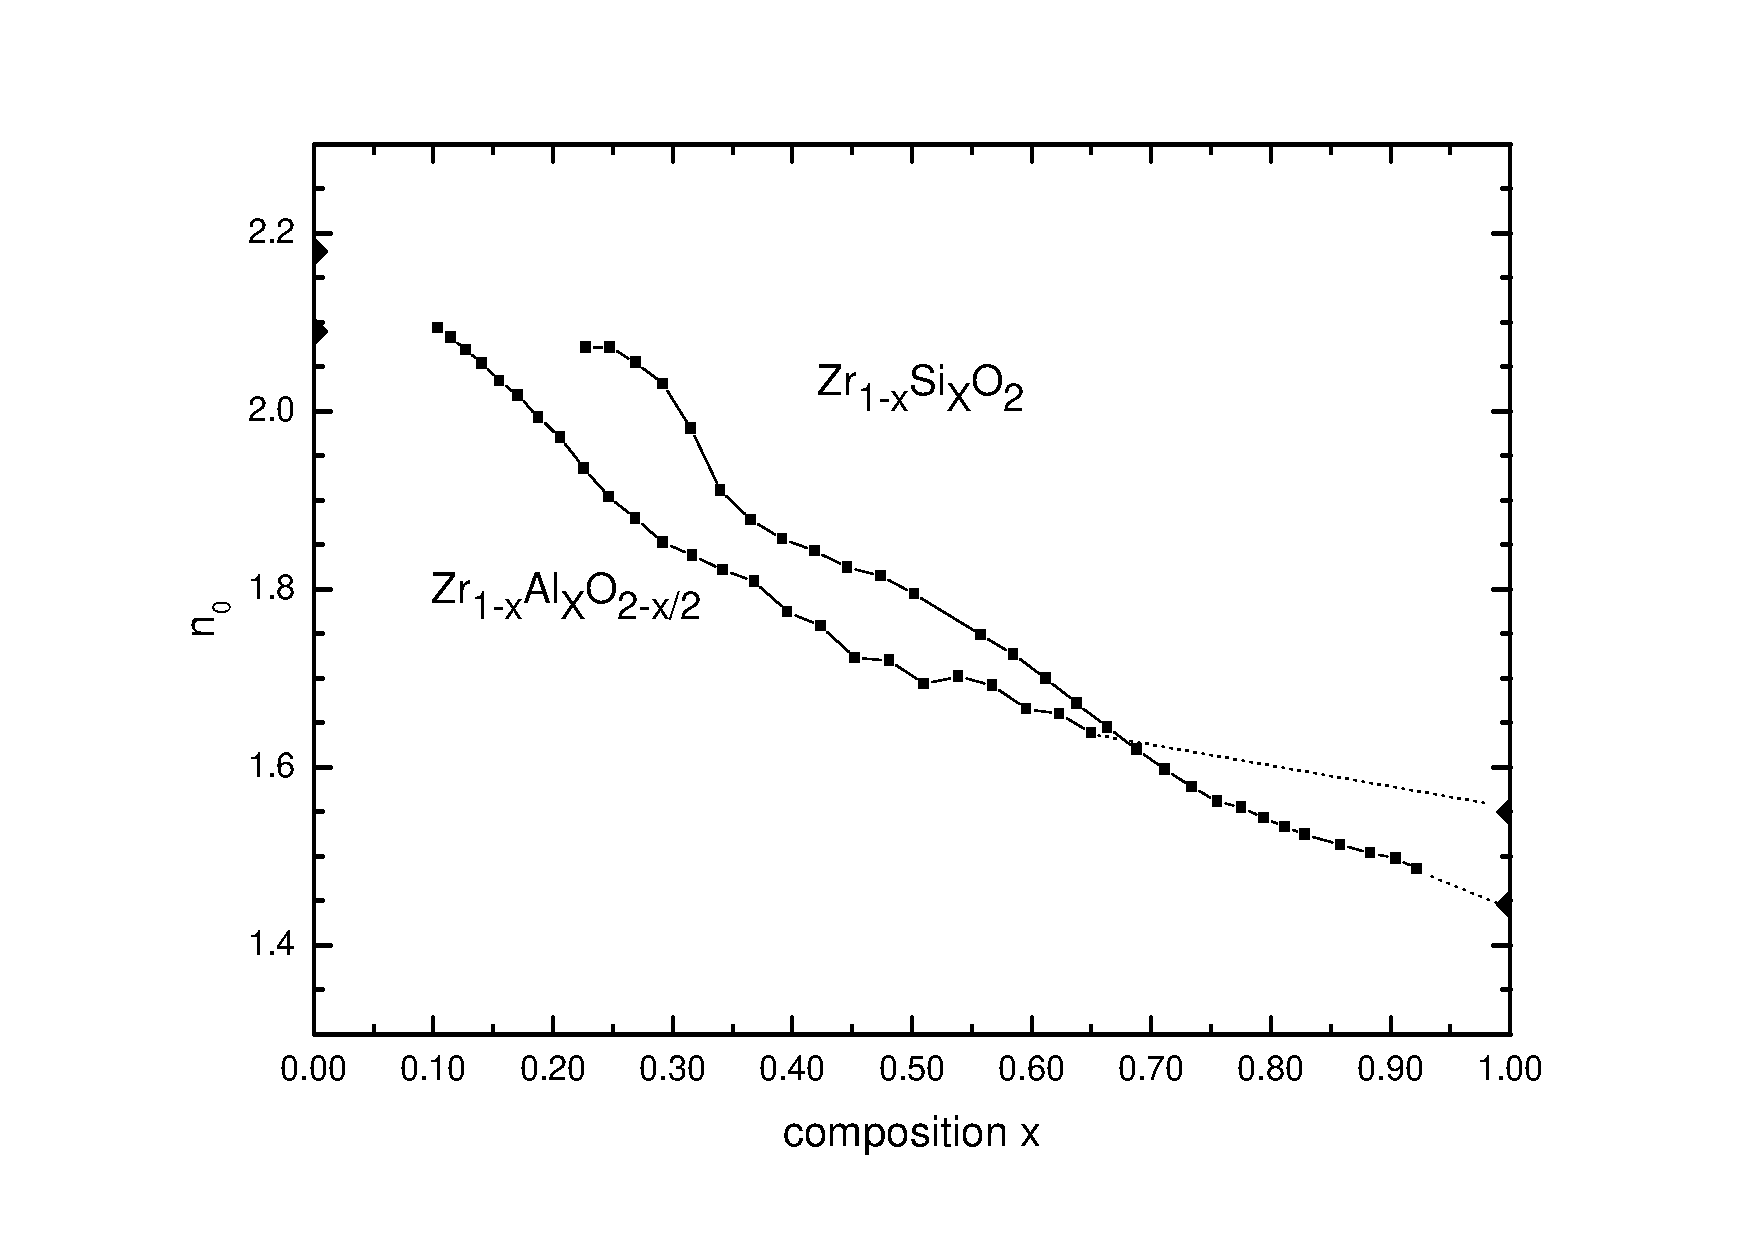
\includegraphics[width=\linewidth]{chapter_3/ZrAlO_ZrSiO_index.pdf}
\caption{Bottom: Composition dependence of the refractive index $n_0$ of thin film
$\textnormal{Zr}_{1-x}\textnormal{Al}_{x}\textnormal{O}_{2-x/2}$ and
$\textnormal{Zr}_{x}\textnormal{Si}_{1-x}\textnormal{O}_{2}$ 
deposited at room temperature. Dotted lines represent extrapolations to values for the endmembers (crystalline and amorphous \ce{ZrO2} and amorphous \ce{SiO2} and \ce{Al2O3}) indicated with triangles.}
\label{ZrAlO_ZrSiO_index}
\end{figure}
%
\subsection{Microscopic picture: static and electronic polarizability}
The high frequency dielectric constant is simply $\varepsilon_{\infty} = n^2$. See supplementary material at [URL will be inserted by AIP] for graphs comparing composition dependence of the static dielectric constant with the $\varepsilon_\infty$. 
But comparing $\varepsilon_s$ with $\varepsilon_{\infty}$ does not offer insight into the behavior at the local level because it does not account for depolarization effects and therefore does not account for density variations correctly. 
Interpreting local polarization behavior in this context does not mean associating a fixed polarizability with specific ions, but is simply a way to compare trends. 
A baseline expectation might be that the composition dependence of the polarizability interpolates linearly between the values for the endmembers. 
Deviations from that trend would suggest unexpected interactions or structural anomalies.

The Clausius-Mossotti equation relates the local polarizability to the externally observed dielectric constant:
$$
\frac{\varepsilon_s -1}{\varepsilon_s +2} = \frac{4 \pi}{3} \sum_{m}{\frac{\alpha_j}{V_m}}
$$
where $\alpha_j$ is the polarizability due to mechanism ${j \in \{electronic, ionic, dipolar, \ldots\}}$,
and $V_m$ is the molar volume.
For the materials under consideration only electronic ($\alpha_e$) and ionic ($\alpha_{ion}$) mechanisms are present. At optical frequencies, well above any phonon modes, only the electronic mechanism is active, so we can infer $\alpha_e /V$ directly from the refractive index. These values are plotted in Figs. \ref{ZrSiO_polariz_over_mol_vol} and \ref{ZrAlO_static_optical_polarizability}, for Zr-Si-O and Zr-Al-O, respectively. 

The data for \ce{SiO2}-rich Zr-Si-O closely follow a simple linear interpolation between the values for the endmembers; the slight deviations are not thought to be meaningful. For  $x < 0.35$ the deviation is significant and is associated with the presence of nanocrystallity. The data for $0.20 < x < 0.30$ are nearly constant, and match the value for unsubstituted \ce{ZrO2}.  We speculate that introduction of \ce{SiO2} decreases the polarizability and the molar volume at compensating rates, leaving $\alpha_e /V$ constant, and that at $x \approx 0.35$ the transition to a disordered structure leads to a fairly abrupt decrease in the molar volume.

The optical polarizability in the Zr-Al-O system follows a significantly different pattern. Here the trend deviates \emph{below} the linear interpolation of endmember values, suggesting either an increased molar volume or an electronic interaction that lowers the polarizability of the system. The data follow a relative smooth curve and extrapolate accurately to the values for the endmembers. In the Zr-Al-O system there is no abrupt transition in $\alpha_e$ associated with the crystalline-amorphous structural transition.     
%
\begin{figure}
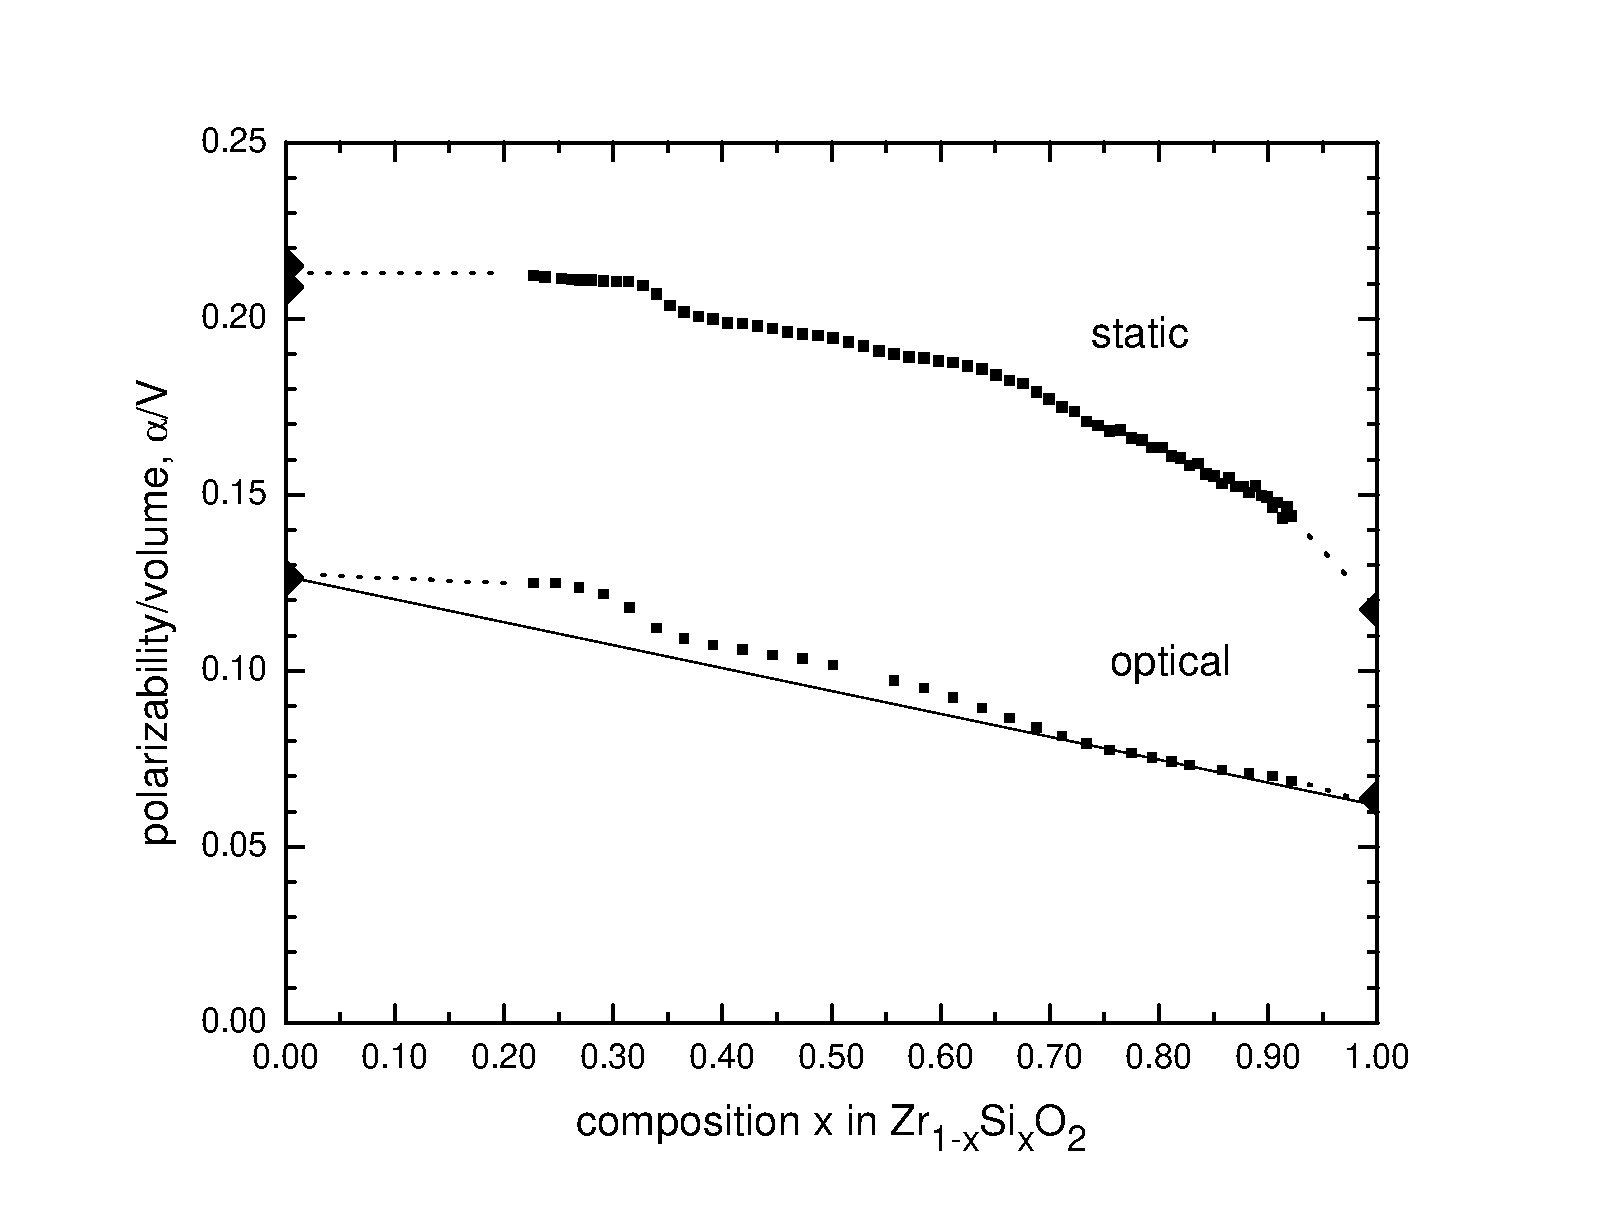
\includegraphics[width=\linewidth]{chapter_3/ZrSiO_polariz_over_mol_vol.pdf}
\caption{Composition dependence of the polarizability per unit volume, $\alpha /V$. Dotted lines are extrapolations to values for the endmembers (crystalline and amorphous \ce{ZrO2} and amorphous \ce{SiO2}) indicated with triangles. Top curve: polarizability inferred from the static (10 kHz) dielectric constant. Bottom curve: polarizability inferred from the optical index of refraction. The solid line is a simple interpolation between the values for the endmembers.}
\label{ZrSiO_polariz_over_mol_vol}
\end{figure}


Figures \ref{ZrSiO_polariz_over_mol_vol} and \ref{ZrAlO_static_optical_polarizability} also show the composition dependence of the static polarizability, $\alpha_s /V$, to which both electronic and ionic mechanisms contribute. In the $\textnormal{Zr}_{1-x}\textnormal{Si}_{x}\textnormal{O}_{2}$ system, $\alpha_s /V$ is nearly constant with increasing \ce{SiO2} fraction until at the crystalline/amorphous there is an abrupt decrease, presumably associated with an increase in molar volume. For $x > 0.35$ the trend of $\alpha_s (x)/V$ shows clear negative curvature, leading to a rapid decrease for the most \ce{SiO2}-rich compositions. In the $\textnormal{Zr}_{1-x}\textnormal{Al}_{x}\textnormal{O}_{2-x/2}$ system a less pronounced decrease is associated with the crystalline/amorphous transition, and there is almost no curvature in $\alpha_s (x)/V$ for $x > 0.35$. Fairly abrupt transitions in both the optical and static polarizability are seen around $x = 0.3$ for both chemical systems, clearly associated with the transitions in the dielectric constant. These might be related to changes in molecular density, or could indicate a change in one of the mechanisms for the polarizability.
%
\begin{figure}
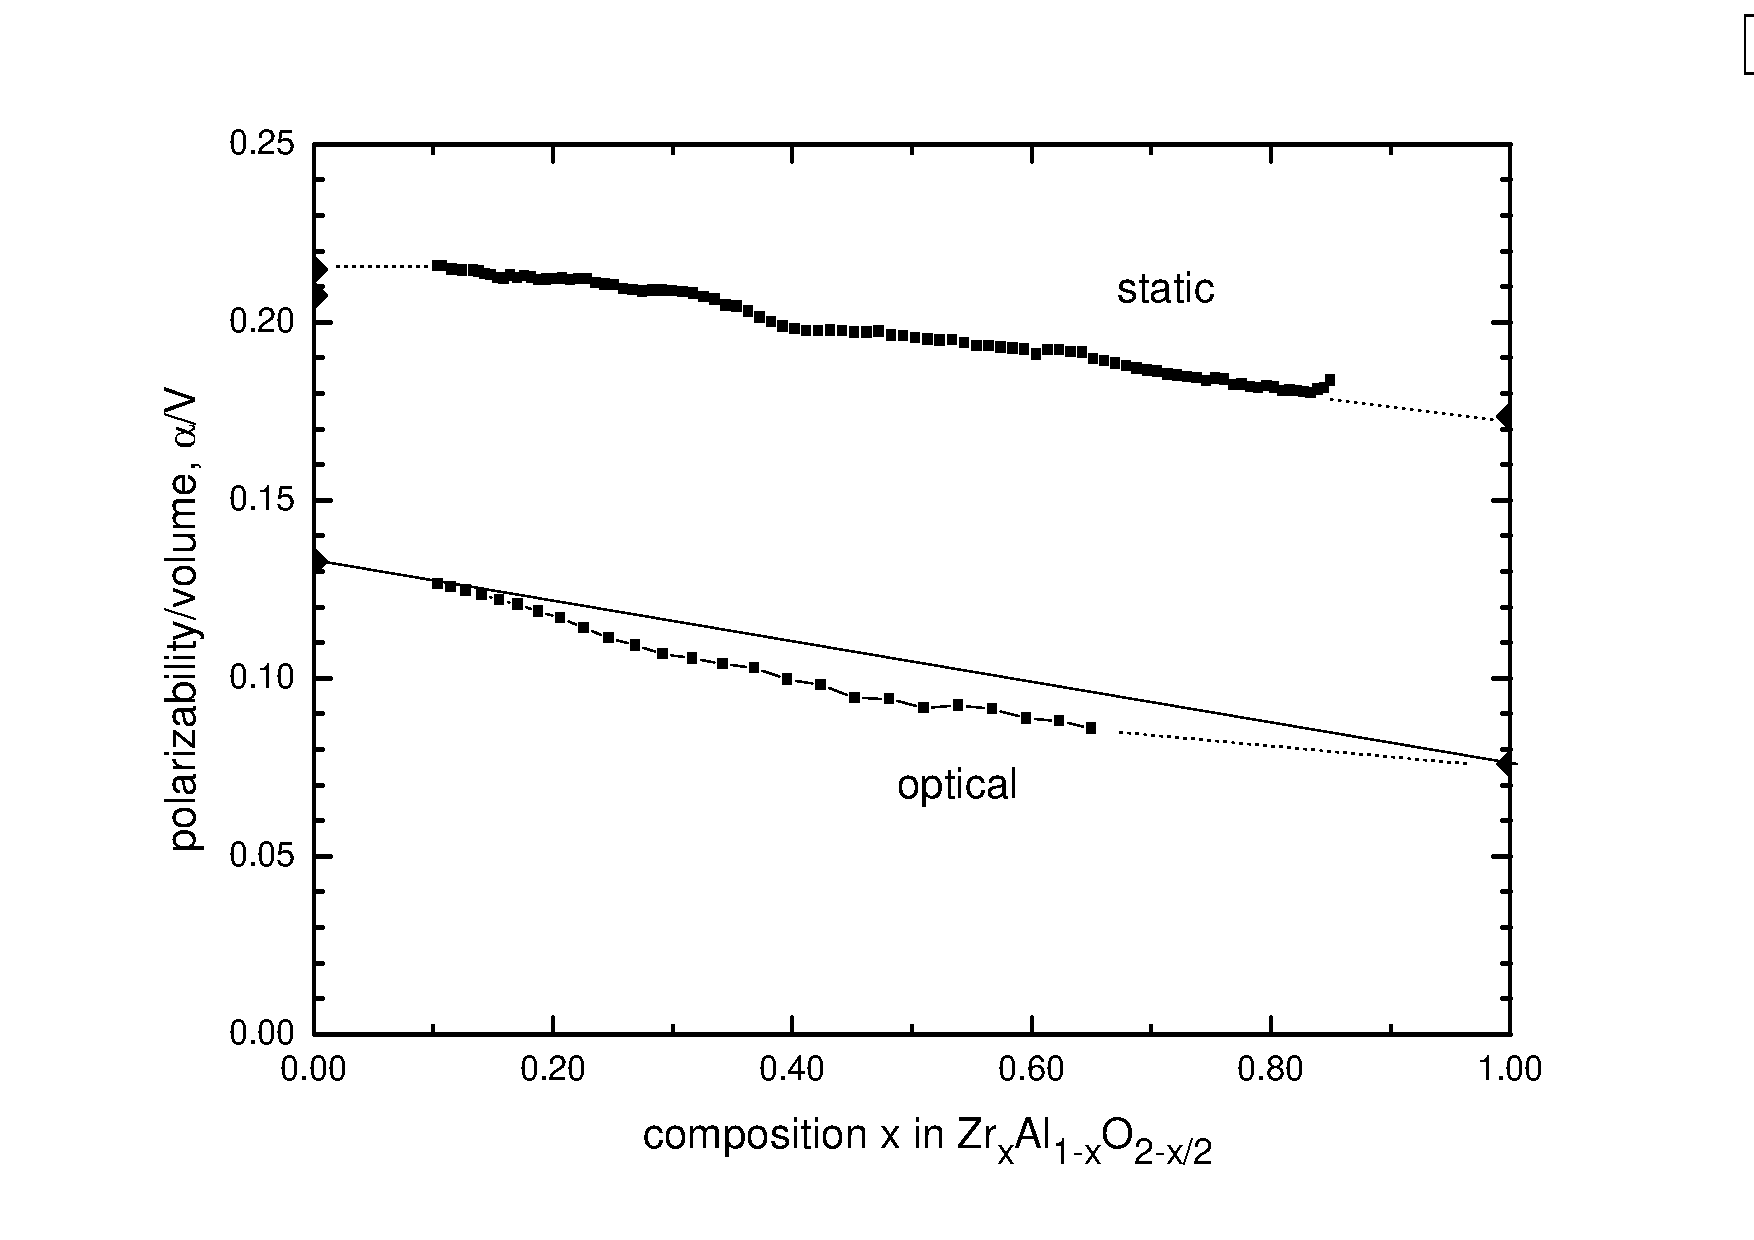
\includegraphics[width=\linewidth]{chapter_3/ZrAlO_static_optical_polarizability.pdf}
\caption{Composition dependence of the polarizability per unit volume, $\alpha /V$. Dotted lines are extrapolations to values for the endmembers (crystalline and amorphous \ce{ZrO2} and amorphous \ce{Al2O3}) indicated with triangles. Top curve: polarizability inferred from the static (10 kHz) dielectric constant. Bottom curve: polarizability inferred from the optical index of refraction. The solid line is a simple interpolation between the values for the endmembers.}
\label{ZrAlO_static_optical_polarizability}
\end{figure}
%
\subsection{Microscopic picture: ionic polarizability}
The difference between the static and optical dielectric responses is due to the displacement of ions, a mechanism that is active only at phonon frequencies and below. Thus the ionic contribution can be inferred using $\alpha_{ionic} /V = \alpha_s /V - \alpha_e /V$. In Fig. \ref{ZrSiO_ZrAlO_diff_polariz} we calculate this difference using the data of Figs. \ref{ZrSiO_polariz_over_mol_vol} and \ref{ZrAlO_static_optical_polarizability}, in which the optical polarizability was interpolated using a cubic spline before subtracting from the static polarizability. Although the data exhibit small wiggles that are probably not meaningful, the two systems demonstrate clearly different trends. The data for both compositions spreads can be seen to extrapolate plausibly to standard values inferred for the endmembers. The Zr-Al-O system exhibits a distinct increase in $\alpha_{ionic} /V (x)$ for increasing $x$ up to $x \approx 0.3 $, after which $\alpha_{ionic} /V$ is nearly independent of $x$. The Zr-Si-O system shows almost the opposite trend: a roughly constant value for $\alpha_{ionic} (x) /V$ for $x < 0.7$ followed by a rapid decrease as the \ce{SiO2} is increased further.
 
At $x = 0.3$, the data $\alpha_{ionic}(x) /V$ in Zr-Al-O do not exhibit a transition comparable to that seen in $\alpha_{e}(x) /V$; only a modest change of overall slope is observed. If the transition in $\alpha_{e}(x) V$ were due to a change in molecular volume $V$, a comparable transition should be observed $\alpha_{ionic}(x) /V$. 
The lack of such a feature implies that the change is in the polarizability $\alpha_e(x)$ at the crystalline/amorphous transition is due to a reorganization of the electron density in the system. 
By comparison, the data for Zr-Si-O are consistent with a model in which the transition is due to a change in molecular volume $V$ rather than $\alpha_{ionic}$ or $\alpha_e$. 

The composition dependence of the dielectric properties of Zr-Al-O and Zr-Si-O follow trends that are subtly but profoundly different, though this is not readily apparent in observations of only the static dielectric constant. 
The main differences are ascribed to substantial changes in bonding and ion dynamics associated with incorporation of \ce{ZrO2} in amorphous \ce{SiO2}-rich Zr-Si-O and incorporation of \ce{Al2O3} in \ce{ZrO2}-rich Zr-Al-O 
(but not with incorporation of \ce{SiO2} in \ce{ZrO2}-rich Zr-Si-O or incorporation of \ce{ZrO2} in amorphous \ce{Al2O3}-rich Zr-Al-O). 
We suggest that this reflects, in the first case, the difference in oxygen coordination for Si (typically tetrahedral) compared to that for Zr (typically octahedral). 
In the second case, it may also reflect the different valence of Al (typically 3$^+$) compared to that of Zr (typically 4$^+$), which would introduce oxygen vacancies to maintain charge neutrality.
The role played by changes in molar volume are not determined in this study, but we speculate that the overall smooth trend in enhancement of the ionic polarizability in Zr-Al-O may be attributed to modest changes in molar volume.
The abrupt change in the polarizability in Zr-Si-O at $\approx$35\% Si can plausibly be attributed to a change in molar volume associated with the crystalline/amorphous transition.
A more conclusive interpretation of the bonding changes would require data from local probes such as EXAFS, or Raman or infrared spectroscopy, coupled with \textit{ab initio} calculations of average structure in the amorphous materials.              
%
\begin{figure}
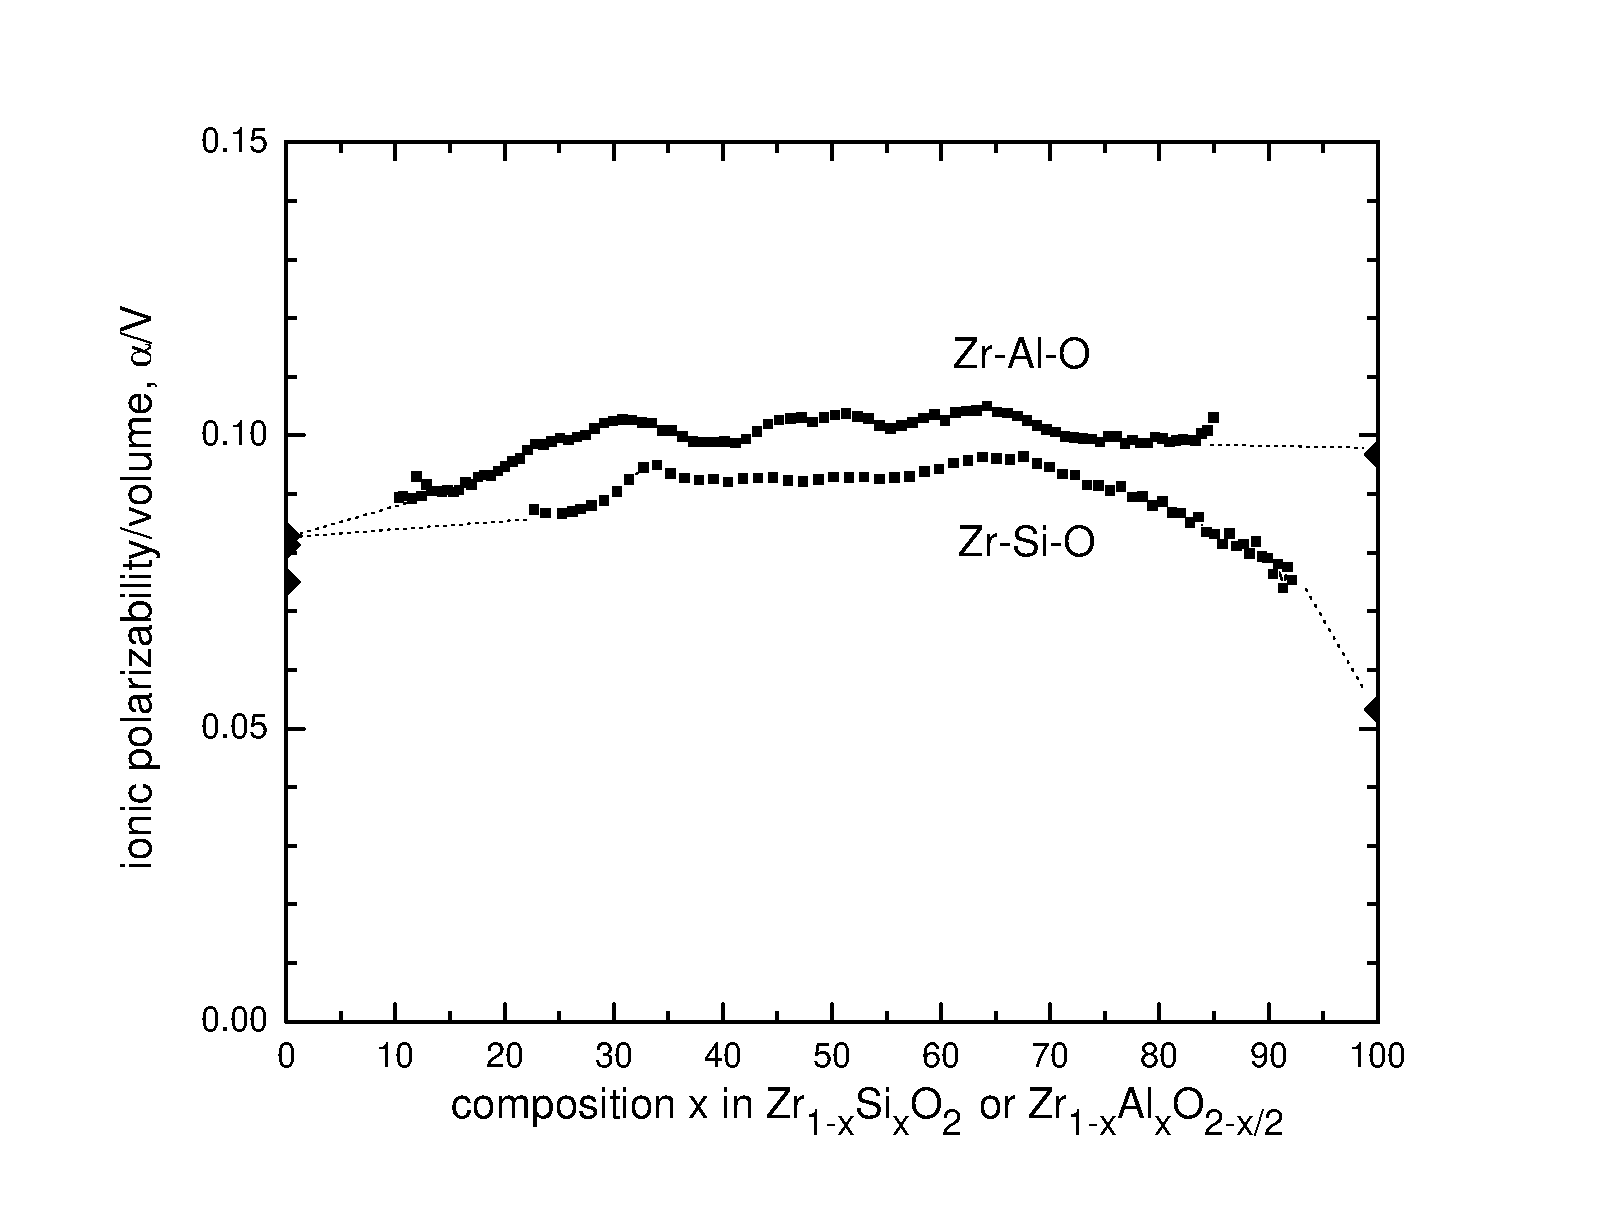
\includegraphics[width=\linewidth]{chapter_3/ZrSiO_ZrAlO_diff_polariz.pdf}
\caption{Composition dependence of the ionic polarizability,, as inferred from the text. Dotted lines represent extrapolations to values for the endmembers (crystalline and amorphous \ce{ZrO2} and amorphous \ce{SiO2} and \ce{Al2O3}) indicated with triangles.} 
\label{ZrSiO_ZrAlO_diff_polariz}
\end{figure}

\subsection{Breakdown field}
The leakage current and breakdown field of these materials is of significant technological interest, as they affect their suitability for any application in which charge or energy storage is important. 
Both properties depend on extrinsic mechanism such as details of impurity concentration, local inhomogeneity, film smoothness, electrode composition, etc., so that few general conclusions can be drawn. 
Fig. \ref{ZrSiAlO_Ebreakdown} presents composition dependence of the breakdown field for $\textnormal{Zr}_{1-x}\textnormal{Al}_{x}\textnormal{O}_{2-x/2}$ and $\textnormal{Zr}_{1-x}\textnormal{Si}_{x}\textnormal{O}_{2}$. For both materials, the breakdown fields range from $\approx 4$ MV/cm for the Zr-rich compositions to $\approx 6$ MV/cm for the Al-rich and Si-rich compositions. 
The significant feature in this data is that in both systems there is no change in breakdown field associated with the crystalline/amorphous transition at $x \approx 0.35$. 
This result clearly repudiates the conventional wisdom that the breakdown field of thin film polycrystalline materials must be compromised due to ``weak'' grain boundaries, as is observed in bulk ceramics. 
As indicated by the crystallite size plotted in Figs. \ref{ZrAlO_epsilon_cohere} and \ref{ZrSiO_eps_cohere}, the films have a high density of grain boundaries. 
This behavior suggests that grain boundaries in the thin films do not act as sinks for impurities and defects during growth, unlike those in high-temperature processed bulk ceramics.       
%
\begin{figure}
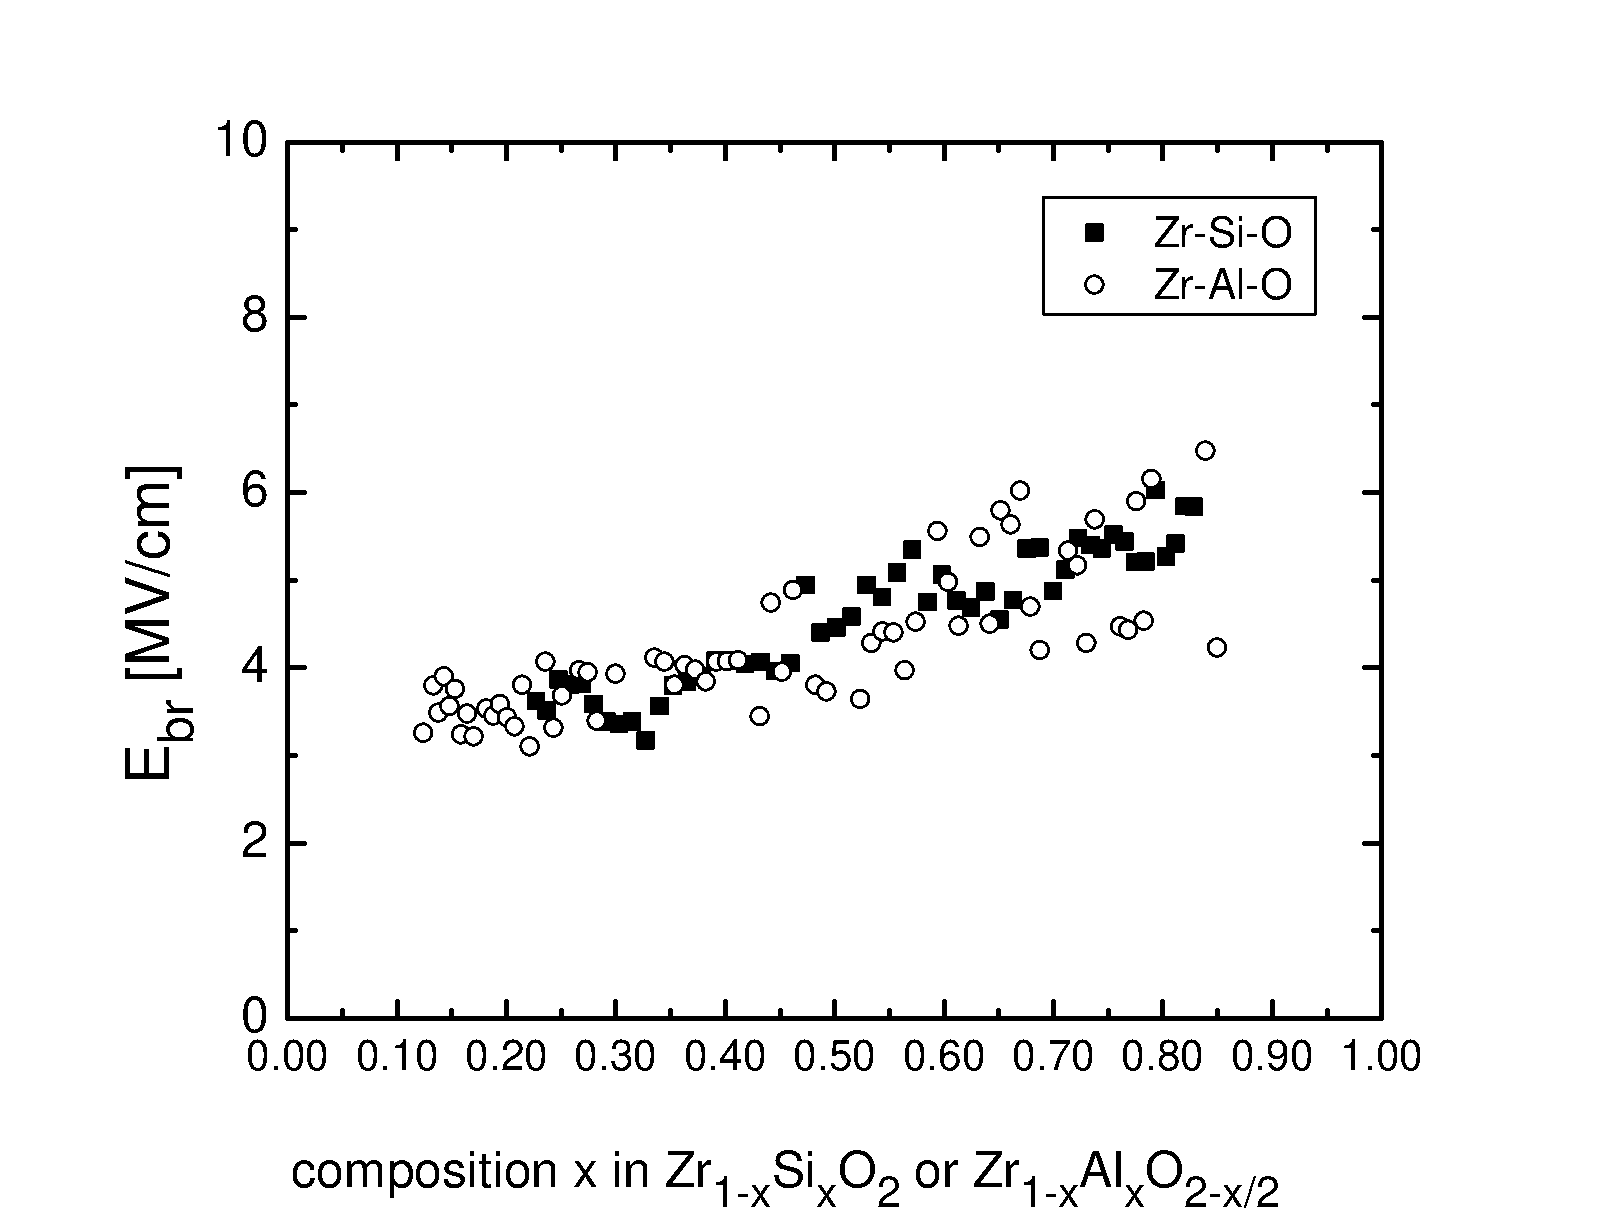
\includegraphics[width=\linewidth]{chapter_3/ZrSiAlO_Ebreakdown.pdf}
\caption{Composition dependence of the breakdown field in Zr-Si-O and Zr-Al-O. Solid symbols represent Zr-Al-O capacitors and open circles represent Zr-Si-O capacitors. Notice that no change in the trend is associated with the crystalline/amorphous transition at $x \approx 0.35$.}
\label{ZrSiAlO_Ebreakdown}
\end{figure}

\section{Conclusion}

This work shows that thin films of mixed transition-metal/p-block oxides, such as Zr-Si-O, are not as simple as they appear at first glance. Enhancement of the composition-dependent polarizability in amorphous \ce{SiO2}-rich Zr-Si-O is definitively confirmed in the data, while a comparable enhancement in \ce{Al2O3}-rich Zr-Al-O is ruled out though an enhanced polarizability in \ce{ZrO2}-rich Zr-Al-O is observed. 
In Zr-Si-O, but not Zr-Al-O, a change in molecular volume appears to be associated with the crystalline/amorphous transition. 
The changes in low-frequency polarizability are most plausibly attributed to changes in ion dynamics (phonon spectrum), suggesting further experiments directly probing the dynamics by IR spectroscopy. 
No significant change in the breakdown field associated with the crystalline vs. amorphous condition.     

\section{Acknowledgments}
This work was supported by the U.S. Department of Energy under Grant No. DE-FG02-06ER06-15. 
This work was performed in part at the Cornell NanoScale Facility, a member of the National Nanotechnology Infrastructure Network, which is supported by the National Science Foundation under Grant No. ECS-0335765. Additionally, this work made use of the Cornell Center for Materials Research facilities with support from the National Science Foundation Materials Research Science and Engineering Center program under Grant No. DMR-0520404. Preliminary data was obtained at Lucent Technologies Bell Labs. The authors thank Dr. R. M. Fleming for collecting and interpreting the RBS data.
